\documentclass[times, 10pt,twocolumn]{article}
\usepackage{mapnoreduce-report-g03}
\usepackage{times}
\usepackage{graphicx}
\usepackage[utf8x]{inputenc}
\usepackage{enumitem}
\usepackage{amsmath}
\usepackage{bm}
\usepackage{wasysym}
\usepackage{amsfonts}%
\usepackage{amssymb}%
\usepackage{graphicx}
\usepackage{fixltx2e}
\usepackage{color}
\usepackage{colortbl}
\usepackage{subfig}
\usepackage{url}
\usepackage{cite}
\usepackage[portuguese, english]{babel}
\usepackage{threeparttable}
\PassOptionsToPackage{hyphens}{url}\usepackage{hyperref}
\usepackage[hyphens]{url}\hypersetup{breaklinks=true}
\usepackage[square,sort,comma,numbers]{natbib}
\usepackage{tabularx}
\usepackage{booktabs}
\usepackage{chngpage}
\usepackage{pdflscape}
\usepackage[table]{xcolor}
\definecolor{lightgray}{gray}{0.9}
\usepackage{tikz}
\usepackage[printonlyused,nolist]{acronym}

\pagestyle{empty}

\begin{document}
	\title{MapNoReduce Platform}

	\author{
        João Pinho\\jpe.pinho@gmail.com\and Diogo Rosa\\
        diogo.m.c.rosa@gmail.com\and Cláudia Filipe\\
        claudia.p.b.filipe@gmail.com\\\\
		Instituto Superior Técnico\\
        Middleware for Distributed Internet Applications\\
        Lisbon, Portugal
    }
	\maketitle
	\thispagestyle{empty}

    % region: acronyms %
    \acrodef{MNRP}{MapNoReduce Platform}

	\begin{abstract}
		This project consists in the design and implementation of \ac{MNRP}, a simplified implementation of the MapReduce middleware and programming model. This platform extracts the input key/value pairs from input files and distributes the Map calls, called Jobs, across multiple machines, the Workers.
		Also, the platform ensures a good performance by monitoring job's progress, detecting faulty or slow machines and rescheduling their tasks on idle machines. That is assured by Job Trackers, which are distributed in this platform, in contrast to the original implementation of MapReduce, where they are centralized. This mechanism was implemented inspired in Facebook's solution—Corona~\cite{ChingFacebook2012}.
		Additionally, in order to test the platform it was developed a PuppetMaster component which allows to control the platform, and also to induce some delays and faults to the system in order to perform some tests and evaluation.
	\end{abstract}

	\section{Introduction}
	MapReduce was introduced by Google in 2004~\cite{GhemawatMR2008} and is currently one of the most popular approaches for large scale data analytics - also thanks to the availability of high quality open-source implementations. When using the MapReduce paradigm, the computation takes a set of input key/value pairs, and produces a set of output key/value pairs. MapReduce users express the computation as two functions: Map and Reduce.
	This project focuses only the Map part, which uses a Map function given by the user and an input set of key/value pairs to produce a set of key/value pairs.
	In \ac{MNRP} the keys are the numbers of the line of the file being read and the values are the content of those lines.
    The Map invocations, called Jobs, are distributed across multiple machines by automatically partitioning the input data into a set of splits of size S. The input splits can be processed in parallel by those machines, named Workers. The system ensures that for each job submitted, all the input data is processed with a good performance through the monitoring of jobs' progress, fault or slow machines detection and reschedule of idle machine's tasks.
	In the original MapReduce implementation these tasks are performed by the JobTracker which is a centralized component. If the JobTracker fails the system can't receive new jobs nor processing pending ones, which can be critical in systems that need high availability.
	Considering JobTracker as a single point of failure~\cite{Kalavri2013}, it is necessary to replicate this component. As it would add complexity to the system and overhead, this project also introduces a new entity, the CoordinationManager, separating cluster resource management from job coordination, which allows the system to focus on make faster scheduling tasks.

	\section{MapNoReduce Architecture}

        \ac{MNRP} is a simplified implementation of the MapReduce middleware and programming model, focused on the Map part. On this simplified version, our work provides a solution to common problems related with the reference architecture of the MapReduce platform. Those problems are related with fault-tolerance, replication and performance and will be discussed in the next sections. Additionally, we added some features that enable the overall testing of the system, such as the ability to run scripts over one or more functional servers or the capacity to monitor the system state while running those scripts.

        \begin{figure}[!h]
            \begin{center}
                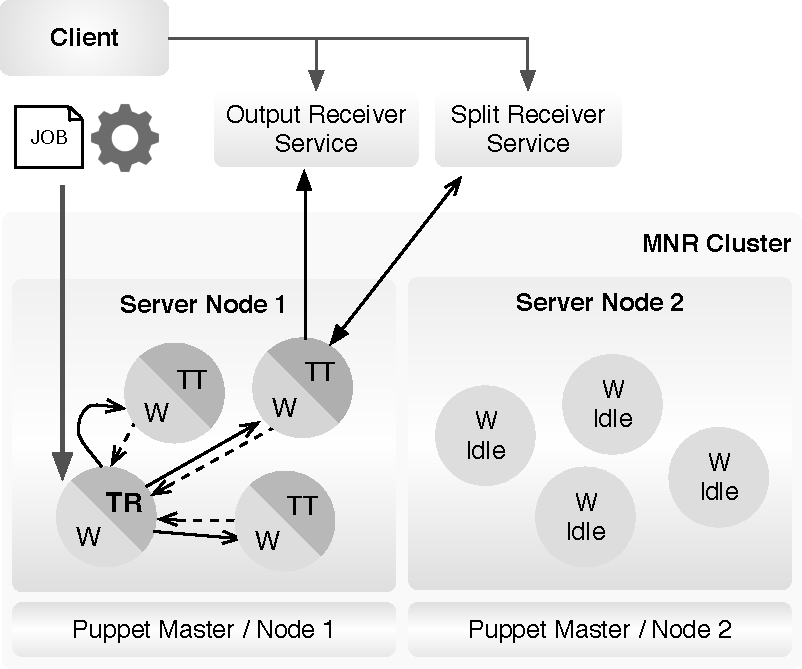
\includegraphics[width=0.48\textwidth]{pics/architecture.pdf}
                \caption{We illustrate an example of the MapNoReduce architecture. We represent one cluster with two server nodes. Inside the processing node, one JobTracker coordinates with other TaskTrackers to process the client job.  }
                \label{fig:mnr-architecture}
            \end{center}
        \end{figure}

    	\subsection{Worker}

        In \ac{MNRP}, workers are simple .NET Remoting Services that receive requests on a given endpoint, known as \emph{Service URI}.

        Every time a job gets submitted to the \ac{MNRP}, an entry worker gets selected to handle its processing. Workers are therefore, available working units that in a given \emph{Server Node} represent its work capacity. This is, for a given server node with 10 workers, such node has capacity to parallelize work to 10 workers.

        The \emph{Service URI} of a worker is composed by 4 parts, starting with the protocol, followed by the \emph{host name}, the \emph{host port}, and finally the worker identifier. An example of such a \emph{Service URI} would be something like \emph{{\small tcp://192.168.1.74:20001/W1}}, representing the endpoint for the worker 1 in the server node.

        It is also worth mentioning that, since a worker is no more than a thread waiting for requests on a given server node — represented by a physical machine, — workers share the same machine resources among them when running in parallel, if all located in the same server node obviously.

        When a worker gets selected by a client application as entry worker, it is made responsible for the correct processing of that job. This means that it must keep track of all the splits that must be processed for that job, what is their status, whose worker is processing each split and in case of a failure it must reassign the lost split to another worker, re-executing the job split if necessary.

        On the other end, each worker that receives the job of processing a given job's split, must report progress to the entry worker in regular intervals, to let it know that the job split is being processed without any problems.

        In the \ac{MNRP}, to an entry worker responsible of managing the processing of a whole job we call, Task Runner and to a worker that reports progress to the Task Runner we call Task Tracker.

    	\subsection{Job Tracker}

        The overall execution and progress tracking of a job is handled by Job Trackers. In \ac{MNRP} \emph{Job Trackers} can have two distinct roles: they could be responsible for the distribution of splits for a given job, or they could be responsible for reporting progress about the processing of a given split.

            \subsubsection{Task Runner}

            When an entry worker receives a job, it is forced to split between two functions: {\it (i)} keep listening for requests for processing new jobs, and {\it (ii)} keep track of the job just received. To achieve the point in {\it (ii)}, the worker creates a \emph{Task Runner} on a new thread, enabling it to keep processing requests without getting blocked while the Task Runner is active.

            Conversely, while the \emph{Task Runner} is actively managing a job, there is no guarantee that no other job arrives during its execution. To avoid blocking incoming requests, we use a FIFO queue, to postpone the execution of jobs received while a job is being handled.

            A \emph{Task Runner} is continuously polling the jobs queue, to check whether it should terminate or process a new job from the queue. In our solution, we decided to terminate the \emph{Task Runner} when there are no jobs, to avoid having a thread wasting resources without any purpose. Because of this, whenever a worker receives a new job it must first determine if it needs to invoke a new \emph{Task Runner} to process the job.

            Finally, the processing of a job can take some time to complete, because of this, the \emph{Task Runner} delegates such processing to a dedicated thread and blocks itself waiting for it to terminate. Note that, the worker thread runs in separate of the \emph{Task Runner}, therefore while the \emph{Task Runner} is blocked its jobs queue can still be updated by the entry worker. The dedicated thread that processes a give job, also known as Job Scheduler is detailed on section \ref{job-scheduler}.

            \begin{figure}[h]
                \begin{center}
                    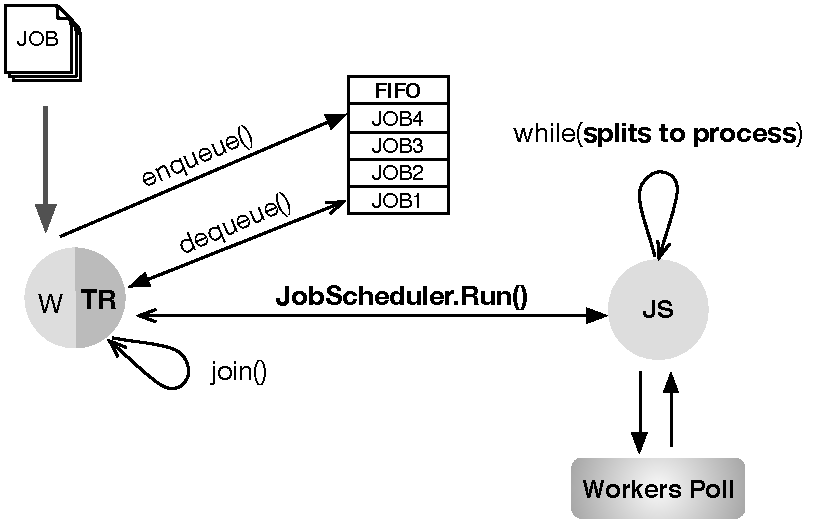
\includegraphics[width=0.48\textwidth]{pics/taskrunner-example.pdf}
                    \caption{A set of jobs are sent to an entry worker. The worker invokes a \textit{TaskRunner}, to enqueue those jobs into a FIFO queue. Then it delegates the first job's execution to a \textit{JobScheduler}, that coordinates with a poll of workers to process the job's splits.}
                    \label{fig:mnr-taskrunner-example}
                \end{center}
            \end{figure}

            \subsubsection{Task Tracker}

           In the \ac{MNRP} every worker can process only one split at a time. Therefore, after receiving a split to process by a given \textit{TaskRunner}, the worker invokes a \textit{TaskTracker} responsible for sending alive signals to the \textit{TaskRunner} with the identifier of the worker that is currently processing a given split. This way the \textit{TaskRunner} can determine if the worker has crashed or if it is stalling the processing of the split — strangler node.

        	\subsubsection{Job Scheduler}\label{job-scheduler}

            \textit{JobScheduler} is responsible for ensuring that all the splits of a given job are processed in order, even in the presence of failures or strangler nodes. To achieve it a \textit{JobScheduler} starts by gathering a set of available workers and distributes the splits among them, in order, i.e, given priority to the splits with a lower number. When a split is delegated to a worker, the scheduler starts tracking the alive signals from that worker and puts that slit in the \textit{SplitsBeingProcessed} queue.

            After the splits distribution procedure finishes, the scheduler computes for every split being processed the time difference, between the workers last alive signal and the current time. For a difference superior to 60 seconds, the worker is assumed to be in a \textit{``not responding''} state, if otherwise the worker is assumed to be processing normally.

            The split processing operation runs asynchronously, i.e, the scheduler delegates the processing of the split to a worker and waits on an asynchronous task, for its response. After completion, the \textit{async} task removes the split from the \textit{SplitsBeingProcessed} queue and marks the worker status as \textit{``available"} for processing more splits.

            For crashed workers or workers that are simply taking too long to send alive signals, either because they have just crashed or simply because their network segment is functioning with high latencies, the scheduler retracts the split delegation from the failing worker and automatically assigns it to a new one if possible, otherwise it gets postpone in a waiting queue.

        \subsection{Replication}

        	\subsubsection{Coordination Manager}

        	\subsubsection{Slave Replica}

    	\subsection{Cluster Resource Management}
      The Cluster resource management was built thinking on maximum resources usage even when the request for them wasn't made by nodes within the same cluster. Some research
      has been done regarding other solutions on resources management on map reduce clusters, but our team was fond to the solution suggested Facebook's solution—Corona~\cite{ChingFacebook2012}.
      A solution for resource management was built based on a simpler version of Facebook's one, this was done by implementing a Fair Share Scheduler(explained later), we're resources could be requested by
      Task Runner's within the same cluster and by other Cluster managers, for this every time a worker is created ne cluter manager must be notified for keeping a register
      of all available workers, the same happens for workers that are on use by Task Runners, so each cluster manager keeps this two records plus a list of other known clusters.
      Given this everytime a Task Runner finishes processing a task it releases the workers assigned to it, this way the Cluster Manager keeps an updated record of available resources.
      When a resource request is made to the Cluster Manager, if there are't enough local resources to answer the request, he queries all Clusters known by himself,
      if the gathered resources from other clusters aren't enough, the request is queued and processed when there are available workers at the local cluster.
      When a resources query is issued from one cluster to the other, the issuing cluster manager request is processed like he is a worker from the local cluster,
      on other words the same amount of resources is given to him as to any other requester worker or cluster manager, regarding the Fair-Share Scheduler algorithm.
      This way of processing requests for resources from other clusters, was designed thinking on maximum resources attribution for all requesting Task Runners on
      distributed clusters. The developed resources attribution solution could've been improved by taking into account time slots took by each resource requester.

      \subsubsection{Fair Share Scheduler}
      After some research on the matter, the Fair-Share algorithm seemed the more balanced solution, both on efficiency and time to develop. So in the developed algorithm
      for resource attribution there was taken into account the known PuppetMaster's and Task Runners. The algorithm is quite simple, on resources request, the number of
      available workers is divided by the number of know PuppetMaster's plus the numbers of TaskRunners, this way as written the previous section on requests issued from
      one cluster to other, the requester is given the same ammount of resources as a worker regarding the Fair-Share algorthm. This way the distributed resources request
      is answered with a larger ammount of resources, that it would be if we're taken into account the workers inside de issuing cluster.
      \subsection{Puppet Master}

	    	\subsection{Puppet Master}
		      %What is it? Why is it necessary? What are their functions?
		      Puppet Master is a component developed for testing \ac{MNRP}. To fully understand the potential of this system, we needed a tool, first to monitoring all the system, second to induce some delays and failures to see how the system behaves. The Puppet Master allows to create workers and get the overall status of the system. Additionally, allows to induce some delay on the whole system or only in some workers and even to simulate some failures freezing workers or its communication, ie, the Job Tracker component.
          \subsubsection{Management Interface}
          The interface of Puppet Master it is provided of a script parsing system, which allows the user to introduce some commands through script that can be processed in batch or step-by-step. The user can load and save his scripts. The interface also has an Help menu that helps to build commands providing their syntax, and for the monitoring it shows up a list of the components of the system, their status and a log window, that was pretty useful on the developing phase and helps to track every action on the system.
          \subsubsection{Create Worker}
          The create worker command instantiates a Worker with a given \emph{ID} and registers it on a given \emph{Service URI} associated to the given \emph{Puppet Master URL}. The full command syntax is:

          \emph{WORKER ID PUPPETMASTER-URL SERVICE-URL ENTRY-URL}

          The last parameter, the \emph{Entry URL}, specifies either if this new worker creation should be notified to the other workers, by calling the worker listening in this URI, or not, if it is left in blank.
          The worker creation also implies the update of the list of available workers of this Puppet Master.
          \subsubsection{Status}

          The status command,

          \emph{STATUS}

          prints the \emph{ID} and \emph{Status} of all workers. This \emph{Status} can be  \emph{Busy} if the worker is processing a job, \emph{Available} if is ready to receive a job, \emph{Frozen} if a Freeze Worker command has been used (see section \ref{freeze}), or \emph{Offline}.

          This information is available on the Monitoring tab of the Management Interface.
                 	
          \subsubsection{Wait and Slow Worker}
			The Wait command allows to induce some delay to the whole system of some given seconds:

            \emph{WAIT SECS}

            and it's used to give some time between two commands, for example. Note that this command is only a emph{Thread.Sleep} to the main thread of Puppet Master.

            As well, the Slow Worker command induces a delay of some seconds to the given worker,

            \emph{SLOWW ID SECS}

			using the emph{Thread.Sleep} to the main thread of that worker. This is used to simulated some slow machines that may delay the whole job processing.

            \subsubsection{Freeze/Unfreeze Worker} \label{freeze}
            The Freeze command is used to simulate some machine that fails, helping us testing the system in a suppose real life scenario. This command:

            \emph{FREEZEW ID}

            disables all the worker components and pauses the processing of requests.
            It was implemented attributing a emph{ManualResetEvent} to every request that is received by the worker, which are set to emph{WaitOne} when a freeze command arrives.

            Only when a unfreeze command is received:

            \emph{UNFREEZEW ID}

            the frozen requests are emph{Set} and the worker returns to work.

            \subsubsection{Freeze/Unfreeze Communication}
            To freeze the communication is to simulate the failure of the JobTracker component, since it is the responsible for it. When a freeze communication command is received

	        \emph{FREEZEC ID}

	        it is used a emph{RemotingServices.Disconect} to avoid the component to receive any messages, as if it has failed.

	        To recovery this component it's used the command

	        \emph{UNFREEZEC ID}

	        which reconnects the component, emph{RemotingServices.Marshal}, and returns to process the frozen requests.

            \subsubsection{Submit}
            Last but not least, the Submit command is the one who allows to simulate the interaction with the client. When a submit command is performed

            \emph{SUBMIT ENTRY-URL FILE OUTPUT S MAP DLL}

            it simulates the request of a client to apply a Map function to a set of data. The client requests to a specific worker, given by the \emph{Entry Url}, to process the data contained in the \emph{File}, dividing it into \emph{S} splits which should be distributed along some workers. The map class is given by the parameter \emph{MAP} which implements the \emph{IMapper} interface whose class library location is given by the \emph{DLL}. In the end, the output files should be in the \emph{OUTPUT} folder.

            When a Submit command is performed, the system runs an \emph{UserApplicationSample}. This application instantiates a \emph{ClientService} to run the \emph{Submit} method.
            When a \emph{ClientService} is instantiated, actually two different services are available: {\it (i)} \emph{ClientSplitProviderService} {\it (ii)} \emph{ClientOutputReceiverService}. The \emph{ClientSplitProviderService} is the service that will provide the splits to the workers. The \emph{ClientOutputReceiverService} is the service that will receive the results of the map function in the end of the job processing.

            After the \emph{ClientService} instantiation and the call of \emph{Submit} method with the given parameters, the client does the \emph{SplitAndSave} of the file to process and saves it to a list that will be also send to the worker, that will be the Master Worker.

            There is a third service in the client side, {\it (iii)} \emph{OutputReadyListener} that will be waiting until the job processing is completed.

            On the Master Worker side, when a job is received it is triggered the Task Runner and the \emph{ScheduleJob} method puts the job into the queue. The Task Runner triggers the \emph{DefaultJobScheduler} which is finally the one who dequeues the job, looks at the splits, looks for the available workers and does the \emph{SplitsDelivery}.

            Each available worker will receive a split to apply the map function. When a worker receives a split, it triggers the Task Tracker which changes the worker's status to Busy and shows that it's alive, asks to the \emph{ClientSplitProviderService} the necessary data to process the split and loads the assembly of the map function. With everything ready, the worker applies the map function to the data, accesses the \emph{ClientOutputReceiverService} and sends the result of its processing.

            Back to the client side, the \emph{OutputReadyListener} that was waiting is \emph{Set} when all the splits' result arrive and those results are written to disk in the \emph{OUTPUT} folder.

            The job was successfully processed.
	\section{Evaluation}

	\section{Conclusions}

	\bibliographystyle{mapnoreduce-report-g03}
	\bibliography{mapnoreduce-rpt-g03}
\end{document}
